%!TEX root = ../dissertation.tex

\chapter{Methods}
\label{methods}

This chapter presents the three most propitious strategies to determine the rotation performed by the eye, and consequently its orientation, when having two sets of matching pixel points on the images captured before and after rotating. Two of these methods are taken from the state of the art, \acrlong{oppr} (section \ref{cha2:opprandsphere}) and \acrlong{grat} (section \ref{einvonrev}), the latter rather modified. The third method, \acrfull{mbpe}, is novel, and as the second, uses the baseline constraint mentioned on section \ref{cha1:problemdef} to its advantage.

It's relevant to note for the following deductions that the baseline length, $\mathbf{b}$ and the intrinsic parameters, $K$, are known values taken from the current eye prototype.

\section{Translation derivation}

Because the current eye prototype is a coupled system, the translation can be obtained through the knowledge of the rotation and the baseline length associated. This length is defined as the distance from the center of the camera's sensor to the center of rotation, as shown on Figure \ref{cha3:detori:translation}.
\begin{figure}[ht]
	\centering
	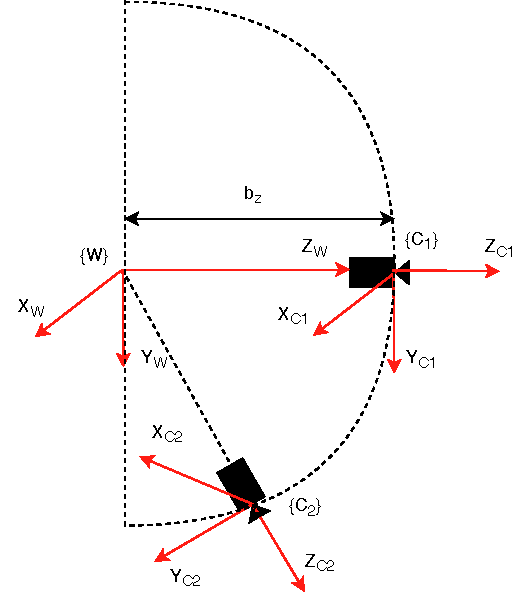
\includegraphics[width=0.5\textwidth]{images/transf.pdf}
	\caption[Translation derivation]{Translation derivation. Effect of a rotation on the current eye prototype's coupled system. The rotation and the baseline length define the translation. ${W}$ is the world reference frame centered on the rotation center, ${C_1}$ is the reference frame of the camera in the first position and ${C_2}$ is its frame on the second position, after rotating. $b_z$ is the baseline length on the Z axis.}
	\label{cha3:detori:translation}
\end{figure}

The translation can be easily derived as follows using frame to frame transformations\footnote{Consult Chapter 2 of Introduction to ROBOTICS mechanics and control \cite{robotics} on Spatial descriptions and transformations}. Having the world reference frame, ${W}$, set at the center of rotation, the transformation from the world to the first position of the camera, ${C_1}$, is
\begin{equation}
^W_{C_1}T = \begin{bmatrix}
I & -\mathbf{b}\\ 
\mathbf{0} & 1
\end{bmatrix},
\end{equation} 
where $I$ is the identity matrix and $\bf b$ is the baseline length expressed in each axis, $X$, $Y$ and $Z$, as $\mathbf{b} = [b_X \ b_Y \ b_Z]$. 
The transformation from the world reference frame to the second position of the camera, ${C_2}$, is
\begin{equation}
^W_{C_2}T = \begin{bmatrix}
R & -\mathbf{b}\\ 
\mathbf{0} & 1
\end{bmatrix},
\end{equation}\\
where $R$ is the rotation.
Hence, the transformation from the first position of the camera to the second can be obtained as
\begin{equation}
^{C_1}_{C_2}T = ^{W}_{C_2}T ^{C_1}_{W}T = ^{W}_{C_2}T ^{W}_{C_1}T^{-1} = 
\begin{bmatrix}
R & -\mathbf{b}\\ 
\mathbf{0} & 1
\end{bmatrix}
\begin{bmatrix}
I & \mathbf{b}\\ 
\mathbf{0} & 1
\end{bmatrix}
=
\begin{bmatrix}
R & R\mathbf{b}-\mathbf{b}\\ 
\mathbf{0} & 1
\end{bmatrix}.
\end{equation}
And finally, the translation ends up as
\begin{equation}
\mathbf{t}(R, \mathbf{b}) = R\mathbf{b}-\mathbf{b} = (R-I)\mathbf{b}.
\end{equation}

\section{\acrlong{mbpe}}
\label{MBaPE}

This algorithm tries to minimize the error between the real image points and its back projections, similarly to algorithm (i) in section \ref{einvonrev}, except that it estimates the variables $R$ and $\mathbf{t}$ directly instead of using the fundamental matrix, $F$, as an intermediate. This seems to prove advantageous in relation to algorithm (i), because solely 3 parameters have to be estimated rather than the whole $F$ matrix. Three parameters are enough to define the rotation (see section \ref{cha2:represent}) and consequently the translation, $\mathbf{t}(R, \mathbf{b})$, as is dependent.\\
It can be seen by the equations \ref{cha2:epipolar:shitshit1} and \ref{cha2:epipolar:shitshit2} used for the re-projections of algorithm (i),
\begin{align}
	\lambda_2 \mathbf{\tilde{m}^r_2} = K [ R \ \mathbf{t} ] K^{-1} \lambda_1 \mathbf{\tilde{m}_1}\\
	\lambda_1 \mathbf{\tilde{m}^r_1} =  K [ R^{T} \ -R^{T}\mathbf{t} ]K^{-1} \lambda_2 \mathbf{\tilde{m}_2},
\end{align}
that $\lambda_1$ and $\lambda_2$, the depth of the corresponding 3D points, is unknown. Therefore, it has to be estimated for each point, making a total of $3+n$ variables to estimate in the minimization.
The cost function to this algorithm is then
\begin{equation}
	\min_{\mathbf{\theta}, \lambda^r_{11}, ..., \lambda^r_{1n}} \sum^n_{i=1} [(u^r_{1i}-u_{1i})^2  + (v^r_{1i}-v_{1i})^2 + (u^r_{2i}-u_{2i})^2 + (v^r_{2i}-v_{2i})^2]
\end{equation}
where $[u_{1i} \ v_{1i}] = \mathbf{m_{1i}}$ are the pixel points in the image before rotating, $[u_{2i} \ v_{2i}] = \mathbf{m_{2i}}$ are the pixel points after rotating, $[u_{1i}^r \ v_{1i}^r] = \mathbf{m_{1i}^r}$ and $[u_{2i}^r \ v_{2i}^r] = \mathbf{m_{2i}^r}$ are its corresponding back projections, $\lambda^r_{11}, ..., \lambda^r_{1n}$ are the estimated depths and $\mathbf{\theta} = [\theta_Z \ \theta_Y \ \theta_X]$ are Euler angles used to determine the rotation.

The back projections should be obtained by
\begin{align*}
	\mathbf{\tilde{m}_{1}^r} = \frac{KR(\mathbf{ \theta})^T(\lambda_{2}^r K^{-1}\mathbf{\tilde{m}_2}) - R(\mathbf{ \theta})^T \mathbf{t}(R(\mathbf{ \theta}), \mathbf{b}))}{\lambda_{1}^r}\\
	\mathbf{\tilde{m}_{2}^r} = \frac{KR(\mathbf{ \theta})(\lambda_{1}^r K^{-1}\mathbf{\tilde{m}_1}) + \mathbf{t}(R(\mathbf{ \theta}), \mathbf{b}))}{\lambda_{2}^r}.
\end{align*} 

In order to start running the algorithm it's necessary to give it initialization parameters, $\lambda_{1}^r$ and $\lambda_{2}^r$ can be acquired from the projection of the image points in a 3D sphere, explained in section \ref{cha2:opprandsphere}, and the Euler angles, $\mathbf{\theta}$, can be given by \acrlong{oppr} as it's a fast and light-weight approximation.

\section{\acrlong{grat}}
On section \ref{cha2:epipolar:fact}, a brief summary explains that to obtain the camera matrix, $R$ and $\mathbf{t}$, using epipolar geometry, the procedure is to determine the fundamental matrix, $F$, followed by determining the essential matrix, $E$, and finally the camera matrix through the \acrshort{svdd} of $E$, choosing the most feasible solution.\\
However, instead of obtaining $R$ and $\mathbf{t}$ through a factorization, this can be estimated rather estimating $F$. Furthermore, given that $\mathbf{t}$ depends on $R$, like before only the 3 parameters have to be estimated. 

These constraint can be used in combination with the most promising epipolar method explained on section \ref{einvonrev}, the \acrlong{grat}. A similar approach is taken by Vasconcelos F. et al \cite{vasconcelos}
to calibrate a camera using multiple sets of pairwise correspondences, in section "8.2 Bundle Adjustment". 

The cost function for this algorithm is then
\begin{align}
\min_\mathbf{\theta} \sum_i \frac{ (\mathbf{\widetilde{\mathbf{m}}_{2i}}^T F \widetilde{\mathbf{m}}_{1i})^2}{\sigma_i^2} \ \text{with}\\
F = K^{-T} [\mathbf{t}]_\times R(\mathbf{ \theta}), K^{-1} \ \text{and}\\
\label{dopewnrvno}
\sigma_i^2 =  [l_{{e1i}_x}^2 + l_{{e1i}_y}^2 + l_{{e2i}_x}^2 + l_{{e2i}_y}^2],
\end{align}
where $\sigma_i^2$ is the variance, $l_{e1i} = F\widetilde{\mathbf{m}}_{2}$ and $l_{e2i} = F\widetilde{\mathbf{m}}_{1}$ are the epipolar lines for each point $i$, $\mathbf{\theta}$ are the Euler angles and $R(\mathbf{ \theta})$ is a rotation matrix obtained through \ref{rrr}. Once again, the initialization of $\mathbf{ \theta}$ can be done using \acrlong{oppr}.\\

As opposed to \acrshort{mbpe}, in \acrshort{grat} the depths of the 3D points are not necessary. An explicit representation of 3D points can be avoided by minimizing the perpendicular distances between point correspondences and their epipolar lines \cite{vasconcelos} \cite{bundle}.
However, because this is based on the fundamental matrix, it won't work for pure rotations, as explained on section \ref{urerrrrr}, where \acrshort{oppr} should prove more suitable. The latter algorithm should yield worst results than the previous two when there is translation associated to the rotation of the eye, as that particularity is ignored.

